\documentclass{standalone}
\usepackage{tikz}
\usetikzlibrary{patterns, positioning}


\begin{document}
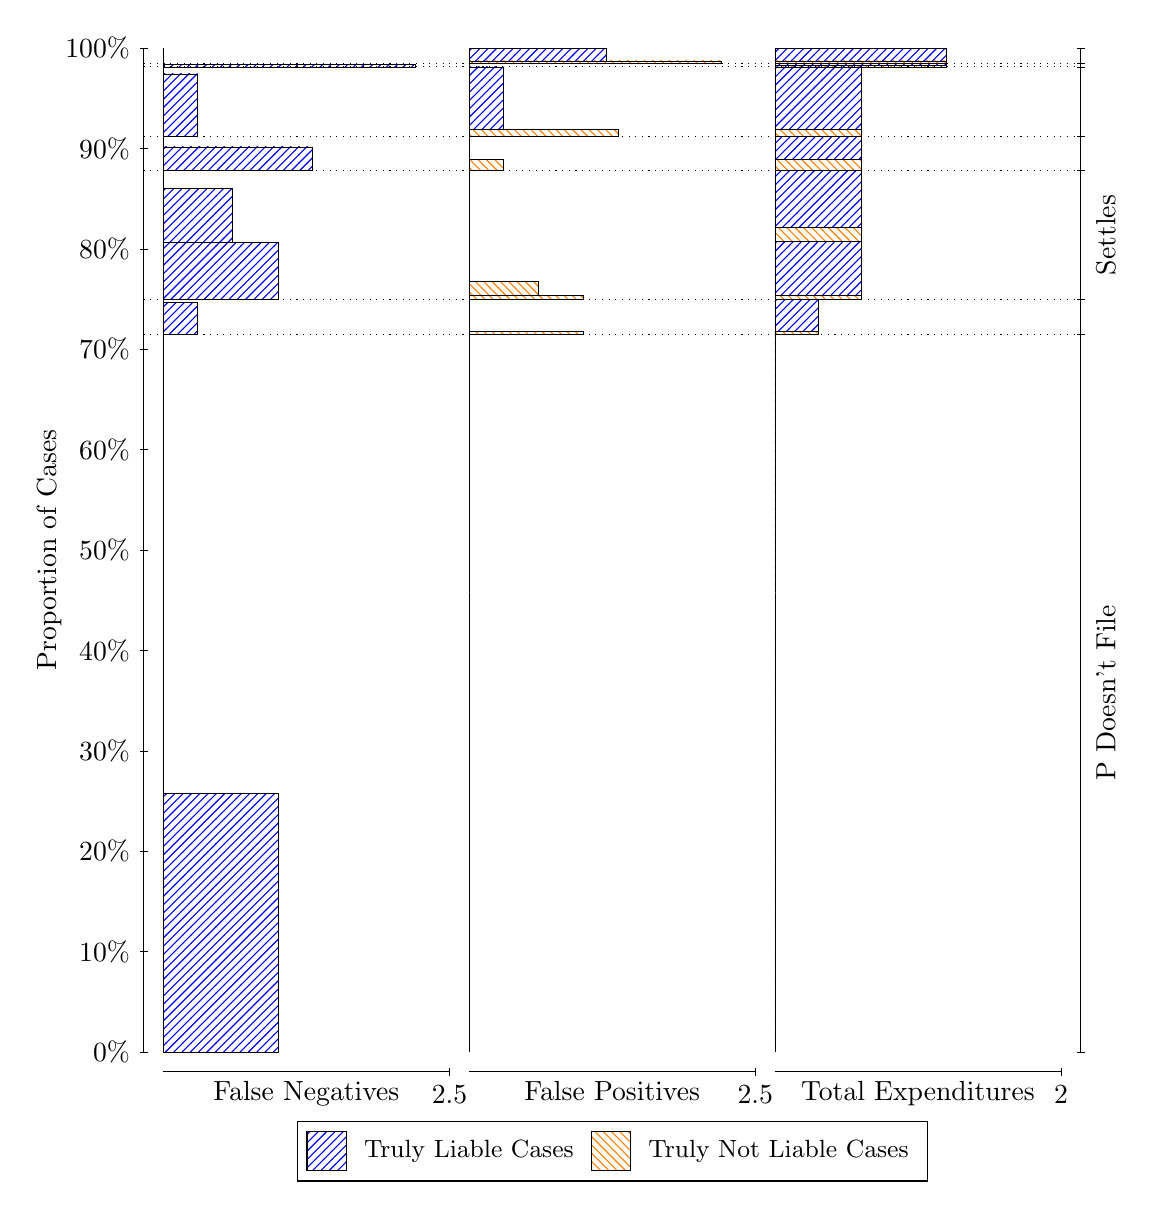
\begin{tikzpicture}
\draw[black, very thin] (1.5,1.75) -- (1.5,14.5);
\node[rotate=90, text=black, anchor=center] at (0.3, 8.125) {Proportion of Cases};
\draw[black, very thin] (1.45,1.75) -- (1.55,1.75);
\node[text=black, anchor=east] at (1.45, 1.75) {0\%};
\draw[black, very thin] (1.45,3.025) -- (1.55,3.025);
\node[text=black, anchor=east] at (1.45, 3.025) {10\%};
\draw[black, very thin] (1.45,4.3) -- (1.55,4.3);
\node[text=black, anchor=east] at (1.45, 4.3) {20\%};
\draw[black, very thin] (1.45,5.575) -- (1.55,5.575);
\node[text=black, anchor=east] at (1.45, 5.575) {30\%};
\draw[black, very thin] (1.45,6.85) -- (1.55,6.85);
\node[text=black, anchor=east] at (1.45, 6.85) {40\%};
\draw[black, very thin] (1.45,8.125) -- (1.55,8.125);
\node[text=black, anchor=east] at (1.45, 8.125) {50\%};
\draw[black, very thin] (1.45,9.4) -- (1.55,9.4);
\node[text=black, anchor=east] at (1.45, 9.4) {60\%};
\draw[black, very thin] (1.45,10.675) -- (1.55,10.675);
\node[text=black, anchor=east] at (1.45, 10.675) {70\%};
\draw[black, very thin] (1.45,11.95) -- (1.55,11.95);
\node[text=black, anchor=east] at (1.45, 11.95) {80\%};
\draw[black, very thin] (1.45,13.225) -- (1.55,13.225);
\node[text=black, anchor=east] at (1.45, 13.225) {90\%};
\draw[black, very thin] (1.45,14.5) -- (1.55,14.5);
\node[text=black, anchor=east] at (1.45, 14.5) {100\%};

\draw[black, very thin] (13.4,1.75) -- (13.4,14.5);
\draw[black, very thin] (13.35,1.75) -- (13.45,1.75);
\node[anchor=west] at (13.35, 1.75) {};
\draw[black, very thin] (13.35,10.866) -- (13.45,10.866);
\node[anchor=west] at (13.35, 10.866) {};
\draw[black, very thin] (13.35,11.303) -- (13.45,11.303);
\node[anchor=west] at (13.35, 11.303) {};
\draw[black, very thin] (13.35,12.947) -- (13.45,12.947);
\node[anchor=west] at (13.35, 12.947) {};
\draw[black, very thin] (13.35,13.379) -- (13.45,13.379);
\node[anchor=west] at (13.35, 13.379) {};
\draw[black, very thin] (13.35,14.261) -- (13.45,14.261);
\node[anchor=west] at (13.35, 14.261) {};
\draw[black, very thin] (13.35,14.308) -- (13.45,14.308);
\node[anchor=west] at (13.35, 14.308) {};
\draw[black, very thin] (13.35,14.5) -- (13.45,14.5);
\node[anchor=west] at (13.35, 14.5) {};

\draw[black, very thin, pattern color=blue, pattern=north east lines] (1.75,1.75) rectangle (3.2033,5.0317);
\draw[black, very thin, pattern color=orange, pattern=north west lines] (1.75,5.0317) rectangle (1.75,10.866);
\draw[black, very thin, pattern color=blue, pattern=north east lines] (1.75,10.866) rectangle (2.186,11.268);
\draw[black, very thin, pattern color=orange, pattern=north west lines] (1.75,11.268) rectangle (1.75,11.303);
\draw[black, very thin, pattern color=blue, pattern=north east lines] (1.75,11.303) rectangle (3.2033,12.027);
\draw[black, very thin, pattern color=blue, pattern=north east lines] (1.75,12.027) rectangle (2.622,12.713);
\draw[black, very thin, pattern color=orange, pattern=north west lines] (1.75,12.713) rectangle (1.75,12.947);
\draw[black, very thin, pattern color=blue, pattern=north east lines] (1.75,12.947) rectangle (3.6393,13.244);
\draw[black, very thin, pattern color=orange, pattern=north west lines] (1.75,13.244) rectangle (1.75,13.379);
\draw[black, very thin, pattern color=blue, pattern=north east lines] (1.75,13.379) rectangle (2.186,14.171);
\draw[black, very thin, pattern color=orange, pattern=north west lines] (1.75,14.171) rectangle (1.75,14.261);
\draw[black, very thin, pattern color=blue, pattern=north east lines] (1.75,14.261) rectangle (4.9473,14.289);
\draw[black, very thin, pattern color=orange, pattern=north west lines] (1.75,14.289) rectangle (1.75,14.308);
\draw[black, very thin, pattern color=orange, pattern=north west lines] (1.75,14.308) rectangle (1.75,14.337);
\draw[black, very thin, pattern color=blue, pattern=north east lines] (1.75,14.337) rectangle (1.75,14.5);
\draw[black, very thin, pattern color=orange, pattern=north west lines] (5.6333,1.75) rectangle (5.6333,7.5844);
\draw[black, very thin, pattern color=blue, pattern=north east lines] (5.6333,7.5844) rectangle (5.6333,10.866);
\draw[black, very thin, pattern color=orange, pattern=north west lines] (5.6333,10.866) rectangle (7.0867,10.9);
\draw[black, very thin, pattern color=blue, pattern=north east lines] (5.6333,10.9) rectangle (5.6333,11.303);
\draw[black, very thin, pattern color=orange, pattern=north west lines] (5.6333,11.303) rectangle (7.0867,11.357);
\draw[black, very thin, pattern color=orange, pattern=north west lines] (5.6333,11.357) rectangle (6.5053,11.536);
\draw[black, very thin, pattern color=blue, pattern=north east lines] (5.6333,11.536) rectangle (5.6333,12.947);
\draw[black, very thin, pattern color=orange, pattern=north west lines] (5.6333,12.947) rectangle (6.0693,13.082);
\draw[black, very thin, pattern color=blue, pattern=north east lines] (5.6333,13.082) rectangle (5.6333,13.379);
\draw[black, very thin, pattern color=orange, pattern=north west lines] (5.6333,13.379) rectangle (7.5227,13.47);
\draw[black, very thin, pattern color=blue, pattern=north east lines] (5.6333,13.47) rectangle (6.0693,14.261);
\draw[black, very thin, pattern color=orange, pattern=north west lines] (5.6333,14.261) rectangle (5.6333,14.28);
\draw[black, very thin, pattern color=blue, pattern=north east lines] (5.6333,14.28) rectangle (5.6333,14.308);
\draw[black, very thin, pattern color=orange, pattern=north west lines] (5.6333,14.308) rectangle (8.8307,14.337);
\draw[black, very thin, pattern color=blue, pattern=north east lines] (5.6333,14.337) rectangle (7.3773,14.5);
\draw[black, very thin, pattern color=orange, pattern=north west lines] (9.5167,1.75) rectangle (9.5167,7.5844);
\draw[black, very thin, pattern color=blue, pattern=north east lines] (9.5167,7.5844) rectangle (9.5167,10.866);
\draw[black, very thin, pattern color=orange, pattern=north west lines] (9.5167,10.866) rectangle (10.062,10.9);
\draw[black, very thin, pattern color=blue, pattern=north east lines] (9.5167,10.9) rectangle (10.062,11.303);
\draw[black, very thin, pattern color=orange, pattern=north west lines] (9.5167,11.303) rectangle (10.607,11.357);
\draw[black, very thin, pattern color=blue, pattern=north east lines] (9.5167,11.357) rectangle (10.607,12.043);
\draw[black, very thin, pattern color=orange, pattern=north west lines] (9.5167,12.043) rectangle (10.607,12.222);
\draw[black, very thin, pattern color=blue, pattern=north east lines] (9.5167,12.222) rectangle (10.607,12.947);
\draw[black, very thin, pattern color=orange, pattern=north west lines] (9.5167,12.947) rectangle (10.607,13.082);
\draw[black, very thin, pattern color=blue, pattern=north east lines] (9.5167,13.082) rectangle (10.607,13.379);
\draw[black, very thin, pattern color=orange, pattern=north west lines] (9.5167,13.379) rectangle (10.607,13.47);
\draw[black, very thin, pattern color=blue, pattern=north east lines] (9.5167,13.47) rectangle (10.607,14.261);
\draw[black, very thin, pattern color=orange, pattern=north west lines] (9.5167,14.261) rectangle (11.697,14.28);
\draw[black, very thin, pattern color=blue, pattern=north east lines] (9.5167,14.28) rectangle (11.697,14.308);
\draw[black, very thin, pattern color=orange, pattern=north west lines] (9.5167,14.308) rectangle (11.697,14.337);
\draw[black, very thin, pattern color=blue, pattern=north east lines] (9.5167,14.337) rectangle (11.697,14.5);
\draw[black, dotted] (1.5,10.866) -- (13.4,10.866);
\draw[black, dotted] (1.5,11.303) -- (13.4,11.303);
\draw[black, dotted] (1.5,12.947) -- (13.4,12.947);
\draw[black, dotted] (1.5,13.379) -- (13.4,13.379);
\draw[black, dotted] (1.5,14.261) -- (13.4,14.261);
\draw[black, dotted] (1.5,14.308) -- (13.4,14.308);
\draw[black, very thin] (1.75,1.5) -- (5.3833,1.5);
\node[text=black, anchor=north] at (3.5667, 1.5) {False Negatives};
\draw[black, very thin] (5.3833,1.45) -- (5.3833,1.55);
\node[text=black, anchor=north] at (5.3833, 1.45) {2.5};

\draw[black, very thin] (5.6333,1.5) -- (9.2667,1.5);
\node[text=black, anchor=north] at (7.45, 1.5) {False Positives};
\draw[black, very thin] (9.2667,1.45) -- (9.2667,1.55);
\node[text=black, anchor=north] at (9.2667, 1.45) {2.5};

\draw[black, very thin] (9.5167,1.5) -- (13.15,1.5);
\node[text=black, anchor=north] at (11.333, 1.5) {Total Expenditures};
\draw[black, very thin] (13.15,1.45) -- (13.15,1.55);
\node[text=black, anchor=north] at (13.15, 1.45) {2};

\node[text=black, centered, rotate=90] at (13.72, 6.308) {P Doesn't File};

\node[text=black, centered, rotate=90] at (13.72, 12.125) {Settles};





\draw (7.449999999999999,1.5) node[draw=none] (baseCoordinate) {};
\begin{scope}[align=center]
        \matrix[scale=0.5, draw=black, below=0.5cm of baseCoordinate, nodes={draw}, column sep=0.1cm]{
            \node[rectangle, draw, minimum width=0.5cm, minimum height=0.5cm, pattern color=blue, pattern=north east lines] {}; &
            \node[draw=none, font=\small, text=black] (B) {Truly Liable Cases}; &
            \node[rectangle, draw, minimum width=0.5cm, minimum height=0.5cm, pattern color=orange, pattern=north west lines] {}; &
            \node[draw=none, font=\small, text=black] (B) {Truly Not Liable Cases}; \\
            };
\end{scope}

\end{tikzpicture}
\end{document}